\documentclass[tikz]{standalone}
\usepackage{fontspec}
\renewcommand*{\familydefault}{\sfdefault}
\usepackage{standalone}
\usepackage{amssymb}
\usetikzlibrary{decorations}
\usetikzlibrary{arrows.meta, decorations.pathmorphing, decorations.pathreplacing, shapes.geometric}
\usetikzlibrary{bayesnet}

\begin{document}

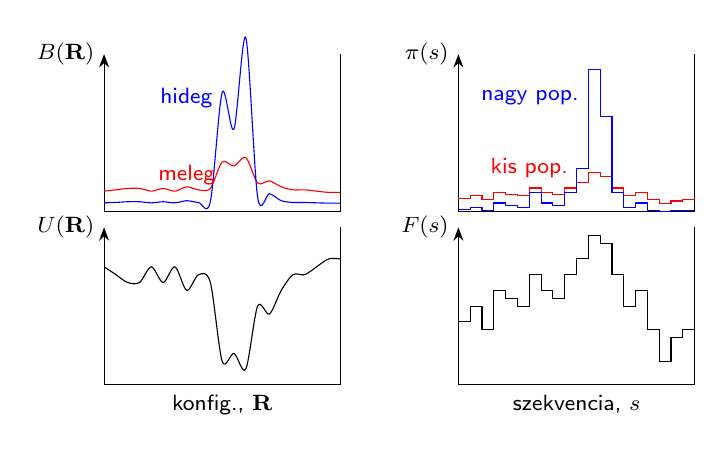
\begin{tikzpicture}[font=\footnotesize, xscale=1.5]

% axes
\draw[-Stealth] (-1,0) -- (-1,2) node[anchor=east] {\(U(\mathbf{R})\)} ;
\draw (1,0) -- (1,2) ;
\draw (-1,0) -- node[anchor=north] {konfig.,~\(\mathbf{R}\)} (1,0) ;

% energy landscape
\draw plot[smooth] coordinates {
(-1.0,1.5) (-0.9,1.4) (-0.8,1.3) (-0.7,1.3) (-0.6,1.5) (-0.5,1.3) (-0.4,1.5)
(-0.3,1.2) (-0.2,1.4) (-0.1,1.3) (0.0,0.3) (0.1,0.4) (0.2,0.2) (0.3,1.0) (0.4,0.9) (0.5,1.2) (0.6,1.4) (0.7,1.4) (0.8,1.5) (0.9,1.6) (1.0,1.6)
};

% fitness landscape
\begin{scope}[xshift=3 cm]

% axes
\draw[-Stealth] (-1,0) -- (-1,2) node[anchor=east] {\(F(s)\)} ;
\draw (1,0) -- (1,2) ;
\draw (-1,0) -- node[anchor=north] {szekvencia, \(s\)} (1,0) (1,0) ;

% fitness landscape
\draw[black] plot[const plot] coordinates {
(-1.0,0.8) (-0.9,1.0) (-0.8,0.7) (-0.7,1.2) (-0.6,1.1) (-0.5,1.0) (-0.4,1.4) (-0.3,1.2) (-0.2,1.1) (-0.1,1.4) (0.0,1.6) (0.1,1.9) (0.2,1.8) (0.3,1.4) (0.4,1.0) (0.5,1.2) (0.6,0.7) (0.7,0.3) (0.8,0.6) (0.9,0.7) (1.0,0.7)
};

\end{scope}

\begin{scope}[yshift=2.2 cm]

% axes
\draw[-Stealth] (-1,0) -- (-1,2) node[anchor=east] {\(B(\mathbf{R})\)} ;
\draw (1,0) -- (1,2) ;
\draw (-1,0) -- (1,0) ;

% Boltzmann distributions

% beta=50
\draw[red, yshift=0.1 cm] plot[smooth] coordinates {
(-1.0,0.16)
(-0.9,0.177)
(-0.8,0.195)
(-0.7,0.195)
(-0.6,0.16)
(-0.5,0.195)
(-0.4,0.16)
(-0.3,0.216)
(-0.2,0.177)
(-0.1,0.195)
(-0.0,0.531)
(+0.1,0.48)
(+0.2,0.587)
(+0.3,0.264)
(+0.4,0.291)
(+0.5,0.216)
(+0.6,0.177)
(+0.7,0.177)
(+0.8,0.16)
(+0.9,0.145)
(+1.0,0.145)
};

% beta=200
\draw[blue, yshift=0.1 cm] plot[smooth] coordinates {
(-1.0,0.012)
(-0.9,0.017)
(-0.8,0.026)
(-0.7,0.026)
(-0.6,0.012)
(-0.5,0.026)
(-0.4,0.012)
(-0.3,0.039)
(-0.2,0.017)
(-0.1,0.026)
(-0.0,1.415)
(+0.1,0.948)
(+0.2,2.11)
(+0.3,0.086)
(+0.4,0.128)
(+0.5,0.039)
(+0.6,0.017)
(+0.7,0.017)
(+0.8,0.012)
(+0.9,0.008)
(+1.0,0.008)
};

% annotations
\path
(0,1.45) node[blue, anchor=east] {hideg}
(-0.3,0.216) node[red, anchor=south] {meleg}
;

% equilibrium measures
\begin{scope}[xshift=3 cm]

% axes
\draw[-Stealth] (-1,0) -- (-1,2) node[anchor=east] {\(\pi(s)\)} ;
\draw (1,0) -- (1,2) ;
\draw (-1,0) -- (1,0) (1,0) ;

% N=50
\draw[red, yshift=-0.0 cm] plot[const plot] coordinates {
(-1.0,0.165)
(-0.9,0.202)
(-0.8,0.149)
(-0.7,0.246)
(-0.6,0.223)
(-0.5,0.202)
(-0.4,0.301)
(-0.3,0.246)
(-0.2,0.223)
(-0.1,0.301)
(-0.0,0.367)
(+0.1,0.496)
(+0.2,0.449)
(+0.3,0.301)
(+0.4,0.202)
(+0.5,0.246)
(+0.6,0.149)
(+0.7,0.1)
(+0.8,0.135)
(+0.9,0.149)
(+1.0,0.149)
};

% equilibrium measure N=200
\draw[blue] plot[const plot] coordinates {
(-1.0,0.022)
(-0.9,0.049)
(-0.8,0.015)
(-0.7,0.11)
(-0.6,0.073)
(-0.5,0.049)
(-0.4,0.244)
(-0.3,0.11)
(-0.2,0.073)
(-0.1,0.244)
(-0.0,0.543)
(+0.1,1.801)
(+0.2,1.207)
(+0.3,0.244)
(+0.4,0.049)
(+0.5,0.11)
(+0.6,0.015)
(+0.7,0.003)
(+0.8,0.01)
(+0.9,0.015)
(+1.0,0.015)
};

% annotations
\path
(0.1,1.45) node[blue, anchor=east] {nagy pop.}
(-0.4,0.301) node[red, anchor=south] {kis pop.}
;

\end{scope}

\end{scope}

\end{tikzpicture}

\end{document}

